% =============================================================================
\chapter{Wigner representation of BEC}
\label{cha:wigner-bec}
% =============================================================================

In this chapter we will apply the functional operator calculus and the functional Wigner transformation from \charef{wigner} along with the transformation theorems from \charef{wigner-spec} to the master equation of the \abbrev{bec} dynamics.
We will discuss the applicability of the truncation approximation, which is required to get rid of the possible negativity of the Wigner functional.
Finally, we will then employ the correspondences from \appref{fpe-sde} to derive the stochastic equations which can be solved numerically.


% =============================================================================
\section{Hamiltonian}
% =============================================================================

The second-quantized Hamiltonian of a $C$-component \abbrev{bec} in $D$ effective dimensions is expressed using quantum field operators $\Psiopf_j^{\dagger}(\xvec)$ and $\Psiopf_j(\xvec)$ defined by~\eqnref{wigner:op-calculus:field}, with the commutators~\eqnref{wigner:op-calculus:commutators}.
\begin{eqn}
\label{eqn:wigner-bec:hamiltonian:H}
	\hat{H} = \int \upd \xvec \sum_{j=1}^C \sum_{k=1}^C \left\{
		\Psiopf_j^{\dagger} K_{jk} \Psiopf_k
		+ \frac{1}{2} \int \upd \xvec^\prime
			\Psiopf_j^\dagger \Psiopf_k^{\prime\dagger}
			U_{jk}(\xvec - \xvec^\prime)
			\Psiopf_j^\prime \Psiopf_k
	\right\}.
\end{eqn}
Here we use the Einstein summation convention of summing over repeated indices.
$U_{jk}$ is the two-body scattering potential, and $K_{jk}$ is the single-particle Hamiltonian:
\begin{eqn}
	K_{jk} = \left(
			-\frac{\hbar^2}{2m} \nabla^2 + \hbar \omega_j + V_j(\xvec)
		\right) \delta_{jk}
		+ \hbar \tilde{\Omega}_{jk}(t),
\end{eqn}
where $V_j$ is the external trapping potential for spin $j$,
$\omega_j$ is the internal energy of spin $j$,
and $\tilde{\Omega}_{jk}$ represents a time-dependent coupling that is used to rotate one spin projection into another.
For details about the source and the concrete form of this term see \secref{bec-noise:mean-field}.

If we impose an energy cutoff $\ecut$ and only take into account low-energy modes of the field,
the general scattering potential $U_{jk}(\xvec - \xvec^\prime)$ can be replaced by the contact potential $U_{jk} \delta(\xvec - \xvec^\prime)$~\cite{Morgan2000}, giving the effective Hamiltonian
\begin{eqn}
\label{eqn:wigner-bec:hamiltonian:effective-H}
	\hat{H} = \int \upd \xvec \sum_{j=1}^C \sum_{k=1}^C \left\{
		\Psiop_j^{\dagger} K_{jk} \Psiop_k
		+ \frac{U_{jk}}{2} \Psiop_j^\dagger \Psiop_k^\dagger \Psiop_j \Psiop_k
	\right\},
\end{eqn}
where $\Psiopf_j^{\dagger}(\xvec)$ and $\Psiopf_j(\xvec)$ are restricted quantum field operators defined by~\eqnref{wigner:op-calculus:restricted-field}, with the commutators~\eqnref{wigner:op-calculus:restricted-commutators}.

For $s$-wave scattering in three dimensions the coefficient is $U_{jk} = 4 \pi \hbar a_{jk} / m$,
where $a_{jk}$ is the scattering length.
Note that in general case the coefficient must be renormalised depending on the grid~\cite{Kokkelmans2002,Sinatra2002}, but the change is small if $dx_{i}\gg a_{jk}$, where $dx_{i}$ is the grid step in dimension $i$.

% =============================================================================
\section{Energy cutoff}
% =============================================================================

As was noted earlier, in order to use contact interactions, an energy cutoff has to be imposed.
We use two different bases in numerical simulations, plane waves and harmonic oscillator modes (see \appref{bases} for details).
Both have analytical expressions for modes and corresponding energies, which makes the selection of the modes straightforward.

Besides being a requirement for using the contact interaction in the Hamiltonian, the energy cutoff has other important functions.
First, it allows one to check for the convergence of integration with respect to decreasing step of the spatial grid.
It effectively separates the propagation in momentum space (which remains constant) from the propagating of the nonlinear parts of the equation in coordinate space (which, hopefully, becomes more precise when the grid step is decreased).
Alternatively, the energy cutoff can work in a different direction, lowering the amount of modes under consideration while keeping the spatial grid constant.
This helps to satisfy the Wigner truncation condition (see \secref{wigner-bec:truncation} for details).

% =============================================================================
\section{Master equation}
% =============================================================================

Hereinafter field operators and wave functions will be assumed to be defined in restricted basis, unless explicitly stated otherwise.
The Markovian master equation for the system with the inclusion of losses can be written as~\cite{Jack2002}
\begin{eqn}
\label{eqn:wigner-bec:master-eqn:master-eqn}
	\frac{d\hat{\rho}}{dt} =
		- \frac{i}{\hbar} \left[ \hat{H}, \hat{\rho} \right]
		+ \sum_{\lvec} \kappa_{\lvec} \int d\xvec
			\mathcal{L}_{\lvec} \left[ \hat{\rho} \right],
\end{eqn}
where $\lvec = (l_1, l_2, \ldots, l_C)$ is a vector containing the number of particles of the corresponding components participating in the interaction, $C$ being the number of components, and we have introduced local Liouville loss terms,
\begin{eqn}
	\mathcal{L}_{\lvec} \left[ \hat{\rho} \right] =
		2\hat{O}_{\lvec} \hat{\rho} \hat{O}_{\lvec}^\dagger
		- \hat{O}_{\lvec}^\dagger \hat{O}_{\lvec} \hat{\rho}
		- \hat{\rho} \hat{O}_{\lvec}^\dagger \hat{O}_{\lvec}.
\end{eqn}
The reservoir coupling operators $\hat{O}_{\lvec}$ are the distinct $n$-fold products of local field annihilation operators, $\hat{O}_{\lvec} = \hat{O}_{\lvec} (\Psiopvec) = \prod_{c=1}^C \Psiop_c^{l_c}$, describing local $(\sum l_c)$-body collision losses.

The master equation allows us to derive an important property.

\begin{theorem}
	\begin{eqn*}
		\frac{d}{dt} \langle \Psiop_j \rangle
		= \mathcal{P}_{\restbasis_j} \left[
			\langle
				-\frac{i}{\hbar} \left(
					K_{jm} \Psiop_m
					+ U_{jm} \Psiop_m^\dagger \Psiop_m \Psiop_j
				\right)
				- \sum_{\lvec} \kappa_{\lvec}
					\frac{\partial \hat{O}_{\lvec}^\dagger}{\partial \Psiop_j^\dagger} \hat{O}_{\lvec}
			\rangle
		\right]
	\end{eqn*}
\end{theorem}
\begin{proof}
\begin{eqn}
	\frac{d}{dt} \langle \Psiop_j \rangle
	={} & \frac{d}{dt} \Trace{ \hat{\rho} \Psiop_j }
	= \Trace{ \frac{d\hat{\rho}}{dt} \Psiop_j } \\
	={} & \Trace{ -\frac{i}{\hbar} \left[ \hat{H}, \hat{\rho} \right] \Psiop_j }
	+ \sum_{\lvec} \kappa_{\lvec} \int d\xvec^\prime
		\Trace{
			\mathcal{L}_{\lvec}^\prime \left[ \hat{\rho} \right]
			\Psiop_j
		} \\
	={} & \int d\xvec^\prime \left(
		- \frac{i}{\hbar} \Trace{
			\left[
				\Psiop_l^{\prime\dagger} K_{lm}^\prime \Psiop_m^\prime,
				\hat{\rho}
			\right] \Psiop_j
		}
		- \frac{i}{2\hbar} U_{lm} \Trace{
			\left[
				\Psiop_l^{\prime\dagger} \Psiop_m^{\prime\dagger}
				\Psiop_l^\prime \Psiop_m^\prime,
				\hat{\rho}
			\right] \Psiop_j
		} \right. \\
	& \left. + \sum_{\lvec} \kappa_{\lvec}
			\Trace{
				\mathcal{L}_{\lvec}^\prime \left[ \hat{\rho} \right]
				\Psiop_j
			}
	\right),
\end{eqn}
where $K_{lm}^\prime \equiv K_{lm}(\xvec^\prime)$, $\mathcal{L}_{\lvec}^\prime \equiv \mathcal{L} [ O_{\lvec}^\prime ] \equiv \mathcal{L} [ O_{\lvec} ( \Psiopvec^\prime ) ]$.

Let us transform each term separately.
We will make extensive use of the fact that trace is invariant under cyclic permutations to re-order the operators in terms.
In addition, the transformations are based on commutation relations proved in \lmmref{op-calculus:functional-commutators}.

Noticing that $[ K_{lm}^\prime, \Psiop_j ] \equiv 0$, the first term can be transformed as:
\begin{eqn}
	\Trace{
		\left[
			\Psiop_l^{\prime\dagger} K_{lm}^\prime \Psiop_m^\prime,
			\hat{\rho}
		\right] \Psiop_j
	}
	& = \Trace{
		\Psiop_l^{\prime\dagger} K_{lm}^\prime \Psiop_m^\prime \hat{\rho} \Psiop_j
		- \hat{\rho} \Psiop_l^{\prime\dagger} K_{lm}^\prime \Psiop_m^\prime \Psiop_j
	} \\
	& = \Trace{
		\hat{\rho} \left(
			\Psiop_j \Psiop_l^{\prime\dagger} K_{lm}^\prime \Psiop_m^\prime
			- \Psiop_l^{\prime\dagger} K_{lm}^\prime \Psiop_m^\prime \Psiop_j
		\right)
	} \\
	& = \Trace{
		\hat{\rho} \left[
			\Psiop_j \Psiop_l^{\prime\dagger}
		\right] K_{lm}^\prime \Psiop_m^\prime
	} \\
	& = \Trace{
		\hat{\rho} \delta_{jl} \delta_{\restbasis_j}(\xvec^\prime - \xvec) K_{lm}^\prime \Psiop_m^\prime
	}
	= \delta_{\restbasis_j}(\xvec^\prime - \xvec) \langle K_{jm}^\prime \Psiop_m^\prime \rangle
\end{eqn}

Second (nonlinear) term:
\begin{eqn}
	U_{lm} \Trace{
		\left[
			\Psiop_l^{\prime\dagger} \Psiop_m^{\prime\dagger}
			\Psiop_l^\prime \Psiop_m^\prime,
			\hat{\rho}
		\right] \Psiop_j
	}
	& = U_{lm} \Trace{
		\Psiop_l^{\prime\dagger} \Psiop_m^{\prime\dagger}
		\Psiop_l^\prime \Psiop_m^\prime \hat{\rho} \Psiop_j
		- \hat{\rho} \Psiop_l^{\prime\dagger} \Psiop_m^{\prime\dagger}
		\Psiop_l^\prime \Psiop_m^\prime \Psiop_j
	} \\
	& = U_{lm} \Trace{
		\hat{\rho} \left(
			\Psiop_j \Psiop_l^{\prime\dagger} \Psiop_m^{\prime\dagger}
			\Psiop_l^\prime \Psiop_m^\prime
			- \Psiop_l^{\prime\dagger} \Psiop_m^{\prime\dagger}
			\Psiop_l^\prime \Psiop_m^\prime \Psiop_j
		\right)
	} \\
	& = U_{lm} \Trace{
		\hat{\rho} \left[
			\Psiop_j, \Psiop_l^{\prime\dagger} \Psiop_m^{\prime\dagger}
		\right] \Psiop_l^\prime \Psiop_m^\prime
	} \\
	& = U_{lm} \Trace{
		\hat{\rho} \delta_{\restbasis_j}(\xvec^\prime - \xvec) \left(
			\delta_{jl} \Psiop_m^{\prime\dagger}
			+ \delta_{jm} \Psiop_l^{\prime\dagger}
		\right) \Psiop_l^\prime \Psiop_m^\prime
	} \\
	& = 2 U_{jm} \delta_{\restbasis_j}(\xvec^\prime - \xvec) \Trace{
		\hat{\rho} \Psiop_m^{\prime\dagger} \Psiop_m^\prime \Psiop_j^\prime
	} \\
	& = 2 U_{jm} \delta_{\restbasis_j}(\xvec^\prime - \xvec) \langle
		\Psiop_m^{\prime\dagger} \Psiop_m^\prime \Psiop_j^\prime
	\rangle
\end{eqn}

The third term, coming from the losses, can be calculated as
\begin{eqn}
	\Trace{
		\mathcal{L}_{\lvec}^\prime \left[ \hat{\rho} \right]
		\Psiop_j
	}
	& = \Trace{
		2 \hat{O}_{\lvec}^\prime \hat{\rho} \hat{O}_{\lvec}^{\prime\dagger} \Psiop_j
		- \hat{O}_{\lvec}^{\prime\dagger} \hat{O}_{\lvec}^\prime \hat{\rho} \Psiop_j
		- \hat{\rho} \hat{O}_{\lvec}^{\prime\dagger} \hat{O}_{\lvec}^\prime \Psiop_j
	} \\
	& = \Trace{
		2 \hat{\rho} \hat{O}_{\lvec}^{\prime\dagger} \Psiop_j \hat{O}_{\lvec}^\prime
		- \hat{O}_{\lvec}^{\prime\dagger} \hat{O}_{\lvec}^\prime \hat{\rho} \Psiop_j
		- \hat{\rho} \hat{O}_{\lvec}^{\prime\dagger} \hat{O}_{\lvec}^\prime \Psiop_j
	} \\
	& = \Trace{
		\hat{\rho} \hat{O}_{\lvec}^{\prime\dagger} \hat{O}_{\lvec}^\prime \Psiop_j
		+ \hat{\rho} \hat{O}_{\lvec}^{\prime\dagger} \Psiop_j \hat{O}_{\lvec}^\prime
		- \hat{\rho} \Psiop_j \hat{O}_{\lvec}^{\prime\dagger} \hat{O}_{\lvec}^\prime
		- \hat{\rho} \hat{O}_{\lvec}^{\prime\dagger} \hat{O}_{\lvec}^\prime \Psiop_j
	} \\
	& = \Trace{
		\hat{\rho} \left[
			\hat{O}_{\lvec}^{\prime\dagger}, \Psiop_j
		\right] \hat{O}_{\lvec}^\prime
	} \\
	& = -\delta_{\restbasis_j}(\xvec^\prime - \xvec) \Trace{
		\hat{\rho} \frac{\partial \hat{O}_{\lvec}^{\prime\dagger}}{\partial \Psiop_j^{\prime\dagger}}
		\hat{O}_{\lvec}^\prime
	} \\
	& = -\delta_{\restbasis_j}(\xvec^\prime - \xvec) \langle
		\frac{\partial \hat{O}_{\lvec}^{\prime\dagger}}{\partial \Psiop_j^{\prime\dagger}}
		\hat{O}_{\lvec}^\prime
	\rangle.
\end{eqn}

Thus the full relation is
\begin{eqn}
	\frac{d}{dt} \langle \Psiop_j \rangle
	& = \int d\xvec^\prime \delta_{\restbasis_j}(\xvec^\prime - \xvec) \left(
		- \frac{i}{\hbar} \langle K_{jm}^\prime \Psiop_m^\prime \rangle
		- \frac{i U_{jm}}{\hbar} \langle
			\Psiop_m^{\prime\dagger} \Psiop_m^\prime \Psiop_j^\prime
		\rangle
		- \sum_{\lvec} \kappa_{\lvec} \langle
			\frac{\partial \hat{O}_{\lvec}^{\prime\dagger}}{\partial \Psiop_j^{\prime\dagger}}
			\hat{O}_{\lvec}^\prime
		\rangle
	\right),
\end{eqn}
which is equivalent to the statement of the theorem.
\end{proof}

% =============================================================================
\section{Wigner truncation}
\label{sec:wigner-bec:truncation}
% =============================================================================

In order to solve operator equation~\eqnref{wigner-bec:master-eqn:master-eqn} with the Hamiltonian~\eqnref{wigner-bec:hamiltonian:effective-H} numerically, we will transform it to an ordinary differential equation using the Wigner transformation from \defref{wigner:mc:w-transformation}.

Namely, the term with $K_{jk}$ is transformed using \thmref{wigner-spec:w-commutator1} and \thmref{wigner-spec:w-laplacian-commutator1} (since $K_{jk}$ is basically a sum of the Laplacian operator and functions of $\xvec$):
\begin{eqn}
	\mathcal{W} \left[ [ \int \upd\xvec \Psiop_j^\dagger K_{jk} \Psiop_k, \hat{\rho} ] \right]
	= \int \upd\xvec \left(
			- \frac{\delta}{\delta \Psi_j} K_{jk} \Psi_k
			+ \frac{\delta}{\delta \Psi_k^*} K_{jk} \Psi_j^*
		\right)
		W,
\end{eqn}
where Wigner function $W = \mathcal{W}[\hat{\rho}]$.
Nonlinear term is transformed with \thmref{wigner-spec:w-commutator2} (assuming the locality of the interaction, and $U_{kj} = U_{jk}$):
\begin{eqn}
\label{eqn:wigner-bec:truncation:full-nonlinear}
	\mathcal{W} \left[
		[
			\int \upd\xvec \frac{U_{jk}}{2}
				\Psiop_j^\dagger \Psiop_k^\dagger \Psiop_j \Psiop_k,
			\hat{\rho}
		]
	\right]
	& = \int \upd\xvec U_{jk} \left(
		\frac{\delta}{\delta \Psi_j} \left(
			- \Psi_j \Psi_k \Psi_k^*
			+ \frac{\delta_{\restbasis_k}(\xvec, \xvec)}{2} ( \delta_{jk} \Psi_k + \Psi_j )
		\right) \right. \\
	&	\left. + \frac{\delta}{\delta \Psi_j^*} \left(
			\Psi_j^* \Psi_k \Psi_k^*
			- \frac{\delta_{\restbasis_k}(\xvec, \xvec)}{2} ( \delta_{jk} \Psi_k^* + \Psi_j^* )
		\right) \right. \\
	&	\left.
			+ \frac{\delta}{\delta \Psi_j}
			\frac{\delta}{\delta \Psi_j^*}
			\frac{\delta}{\delta \Psi_k}
			\frac{1}{4} \Psi_k
			- \frac{\delta}{\delta \Psi_j}
			\frac{\delta}{\delta \Psi_j^*}
			\frac{\delta}{\delta \Psi_k^*}
			\frac{1}{4} \Psi_k^*
		\right) W.
\end{eqn}
Loss operator is transformed with \thmref{wigner-spec:w-losses} and result in a similar equation, with a finite number of differential terms up to order $2n$ for $n-$body collisional losses.

Assuming that $K_{jk}$, $U_{jk}$, and $\kappa_{\lvec}$ are real-valued, all the transformations described above result in a partial differential equation for $W$ of the form
\begin{eqn}
\label{eqn:wigner-bec:truncation:untruncated-fpe}
	\frac{\upd W}{\upd t}
	= \int \upd\xvec \left\{
		- \sum_{j=1}^{C} \frac{\fdelta}{\fdelta \Psi_j} \mathcal{A}_j
		- \sum_{j=1}^{C} \frac{\fdelta}{\fdelta \Psi_j^*} \mathcal{A}_j^*
		+ \sum_{j=1}^{C} \sum_{k=1}^{C}
			\frac{\fdelta^2}{\fdelta \Psi_j^* \fdelta \Psi_k} \mathcal{D}_{jk}
		+ \mathcal{O} \left[ \frac{\fdelta^3}{\fdelta \Psi_j^3} \right]
	\right\} W.
\end{eqn}
Terms of order higher than $2$ are produced both by the nonlinear term in the Hamiltonian, and loss terms.
Such an equation could be solved perturbatively if there were only orders up to $3$ (which means an absence of nonlinear losses)~\cite{Polkovnikov2003}, but in most cases all terms except for first- and second-order ones are truncated.
In order to justify this truncation in a consistent way, we develop an order-by-order expansion in $1/N_j$, where $N_j$ is a characteristic particle number in a physical interaction volume, and truncate terms of formal order $1/N_j^2$.
This is achieved by use of the formal definition of a scaled Wigner function $W^{\psi}$~\cite{Drummond1993}, satisfying a scaled equation in terms of dimensionless scaled fields $\psi$, with:
\begin{eqn}
	\tau & = t / t_c, \\
	\psi_{j} & = \Psi_{j}\sqrt{\ell_c / N_j}, \\
	\mathcal{A}_j^{\psi} & = t_c \sqrt{\ell_c / N_j} \mathcal{A}_j
		+ \mathcal{O} \left( 1 / N_j^2 \right), \\
	\mathcal{D}_{jk}^{\psi} & = t_c \left( \ell_c / N_j \right) \mathcal{D}_{jk}
		+ \mathcal{O} \left( 1 / N_j^2 \right).
\end{eqn}
Here $t_c$ is a characteristic interaction time and $\ell_c$ is a characteristic interaction length.
These would normally be chosen as the healing time and healing length respectively in a \abbrev{bec} calculation.
Typically the cell size is chosen as proportional to the healing length, for optimum accuracy in resolving spatial detail.
Using this expansion, a consistent order-by-order expansion in $1/N_j$ can be obtained,
of form:
\begin{eqn}
	\frac{\upd W^{\psi}}{\upd \tau}
	= \int \upd\xvec \left\{
		- \sum_{j=1}^C \frac{\fdelta}{\fdelta \psi_j} \mathcal{A}_j^{\psi}
		- \sum_{j=1}^C \frac{\fdelta}{\fdelta \psi_j^*} \mathcal{A}_j^{\psi*}
		+ \sum_{j=1}^C \sum_{k=1}^C \frac{\fdelta^2}{\fdelta \psi_j^* \fdelta \psi_k}
			\mathcal{D}_{jk}^{\psi}
		+ \mathcal{O} \left[ \frac{1}{N_j^2} \right]
	\right\} W^{\psi}.
\end{eqn}

With the assumption of the state being coherent, the simple condition for truncation~--- that is, omitting terms of the order $\mathcal{O}(1/N_j^2)$~--- can be shown to be~\cite{Sinatra2002}
\begin{eqn}
	N_j \gg |\restbasis_j|,
\end{eqn}
where $N_j$ is the total number of atoms of the component $j$.
The inclusion of the mode factor is caused by the fact that the number of additional terms increases as the number of modes increases, which may be needed to treat convergence of the method for large momentum cutoff.
We see immediately that there are subtleties involved if one wishes to include larger numbers of high-momentum modes, since this increases the mode number while leaving the numbers unchanged.
In other words, the truncation technique is inherently restricted in its ability to resolve fine spatial details in the high-momentum cutoff limit.

The $1/N_j$ is equivalent to an expansion in the inverse density, which requires the inequality~\cite{Norrie2006}
\begin{eqn}
\label{eqn:wigner-bec:truncation:delta-condition}
	\delta_{\restbasis_j}(\xvec, \xvec)
	\ll |\Psi_j|^2.
\end{eqn}
The coherency assumption does not, of course, encompass all possible states that can be produced during evolution, which means that the condition above is more of a guide than a restriction.
For certain systems the truncation was shown to work even when~\eqnref{wigner-bec:truncation:delta-condition} is violated~\cite{Ruostekoski2005}.
The validity may also depend on the simulation time~\cite{Javanainen2013}, and other physically
relevant factors.

A common example of such relevant factors is that there can be a large difference in the size of the original parameters.
To illustrate this issue, one may have a situation where $\kappa_1 \approx \kappa_2 N_j$ even though $N_j \gg 1$.
Under these conditions, it is essential to include a scaling of the parameters in calculating the formal order, so that the scaled parameters have comparable sizes.
This allows one to identify correctly which terms are negligible in a given physical problem, and which terms must be included.

In general, one can estimate the validity of truncation for the particular problem and the particular observable by calculating the quantum correction~\cite{Polkovnikov2010}.
Other techniques for estimating validity include comparison with the exact positive-P simulation method~\cite{Drummond1993}, and examining results for unphysical behaviour such as negative occupation numbers~\cite{Deuar2007}.
It is generally the case for unitary evolution that errors caused by truncation grow in time, leading to a finite time horizon for applicability, as explained in the introduction.

The use of this Wigner truncation allows us to simplify the results of \thmref{wigner-spec:w-commutator2} and \thmref{wigner-spec:w-losses}.
Wigner truncation is an expansion up to the order $1/N_j$, so during the simplification, along with the higher order derivatives, we drop all components with $\delta_{\restbasis_j}$ of order higher than $1$ in the drift terms, and of order higher than $0$ in the diffusion terms.

\begin{theorem}
Assuming the conditions for Wigner truncation are satisfied, the result of the Wigner transformation of the nonlinear term is
\begin{eqn*}
	\mathcal{W} \left[
		[
			\int \upd\xvec \frac{U_{jk}}{2}
				\Psiop_j^\dagger \Psiop_k^\dagger \Psiop_j \Psiop_k,
			\hat{\rho}
		]
	\right]
	\approx{} & \int \upd\xvec U_{jk} \left(
		\frac{\fdelta}{\fdelta \Psi_j} \left(
			- \Psi_j \Psi_k \Psi_k^*
			+ \frac{\delta_{\restbasis_k}(\xvec, \xvec)}{2} ( \delta_{jk} \Psi_k + \Psi_j )
		\right) \right. \\
	&	\left. + \frac{\fdelta}{\fdelta \Psi_j^*} \left(
			\Psi_j^* \Psi_k \Psi_k^*
			- \frac{\delta_{\restbasis_k}(\xvec, \xvec)}{2} ( \delta_{jk} \Psi_k^* + \Psi_j^* )
		\right) \right) W.
\end{eqn*}
\end{theorem}
\begin{proof}
A straigtforward result of neglecting high-order terms in~\eqnref{wigner-bec:truncation:full-nonlinear}.
\end{proof}

\begin{theorem}
Assuming the conditions for Wigner truncation are satisfied, the result of the Wigner transformation of the loss term is
\begin{eqn*}
	\mathcal{W}[\mathcal{L}_{\lvec}[\hat{\rho}]]
	\approx{} & \left(
		\sum_{m=1}^C \frac{\fdelta}{\fdelta\Psi_m^*}
		\left(
			\frac{\upp O_{\lvec}}{\upp \Psi_m} O_{\lvec}^*
			- \frac{1}{2} \sum_{n=1}^{C} \delta_{\restbasis_n}(\xvec, \xvec)
				\frac{\upp^2 O_{\lvec}}{\upp\Psi_m \upp\Psi_n}
				\frac{\upp O_{\lvec}^*}{\upp\Psi_n^*}
		\right)
	\right. \\
	& + \sum_{m=1}^C \frac{\fdelta}{\fdelta\Psi_m}
	\left(
		\frac{\upp O_{\lvec}^*}{\upp \Psi_m^*} O_{\lvec}
		- \frac{1}{2}\sum_{n=1}^C \delta_{\restbasis_n}(\xvec, \xvec)
			\frac{\upp^2 O_{\lvec}^*}{\upp\Psi_m^* \upp\Psi_n^*}
			\frac{\upp O_{\lvec}}{\upp\Psi_n}
	\right) \\
	& \left. + \sum_{m=1}^C \sum_{n=1}^C
		\frac{\fdelta^2}{\fdelta\Psi_m^* \fdelta\Psi_n}
		\frac{\upp O_{\lvec}}{\upp\Psi_m} \frac{\upp O_{\lvec}^*}{\upp\Psi_n^*}
	\right) W,
	\end{eqn*}
where coupling functionals $O_{\lvec} \equiv O_{\lvec}[\Psivec] = \prod_{c=1}^C \Psi_c^{l_c}$.
\end{theorem}
\begin{proof}
The proof is basically a simplification of the result of \thmref{wigner-spec:w-losses} under two conditions following from neglecting the terms smaller than $1 / N$.
First, we are dropping all terms with high order differentials, which can be expressed as limiting $\sum j_c + \sum k_c \le 2$.
Second, we are only considering the terms with the restricted delta function of up to first order in the drift part (containing the functional differentials of order $1$), and terms with no restricted delta functions in the diffusion part (containing the functional differentials of order $2$).

The only combinations of $j_c$ and $k_c$ for which $Z_{\lvec,\jvec,\kvec}$ is not zero are thus $\{ j_c = \delta_{cm}, k_c = 0, m \in [1, C] \}$, $\{ j_c = 0, k_c = \delta_{cm}, m \in [1, C] \}$ and $\{ j_c = \delta_{cm}, k_c = \delta_{cn}, m \in [1, C], n \in [1, C] \}$.
These combinations produce terms with $\frac{\delta}{\delta \Psi_n^*}$, $\frac{\delta}{\delta \Psi_n}$ and $\frac{\delta^2}{\delta \Psi_p \delta \Psi_n^*}$ respectively:
\begin{eqn}
\label{eqn:wigner-bec:truncation:truncated-losses}
	\mathcal{W}[\mathcal{L}_{\lvec}[\hat{\rho}]]
	\approx{} & \left(
		\sum_{m=1}^C \frac{\fdelta}{\fdelta \Psi_m^*} H[l_m - 1] Z_{\lvec, \evec_m, \mathbf{0}}
		+ \sum_{m=1}^C \frac{\fdelta}{\fdelta \Psi_m} H[l_m - 1] Z_{\lvec, \mathbf{0}, \evec_m}
	\right. \\
	& \left. + \sum_{m=1}^C \sum_{n=1}^C \frac{\fdelta^2}{\fdelta \Psi_m^* \fdelta \Psi_n^*}
			H[l_m - 1] H[l_n - 1] Z_{\lvec, \evec_m, \evec_n}
	\right) W,
\end{eqn}
where $\evec_n$ is a vector consisting of zeros and a single $1$ at the $n$-th position, and $H[n]$ is the discrete Heavyside function.

Evaluating the partially parametrized $Z$ function in the first term using the expression in \thmref{wigner-spec:w-losses}:
\begin{eqn}
	Z_{\lvec, \evec_m, \mathbf{0}}
	= l_m \prod_{c=1}^C
		\exp \left(
			-\frac{\delta_{\restbasis_c}(\xvec, \xvec)}{2}
			\frac{\upp^2}{\upp \Psi_c \upp \Psi_c^*}
		\right)
		\Psi_c^{l_c - \delta_{cm}} (\Psi_c^*)^{l_c}.
\end{eqn}
Expanding the exponent in series and discarding the terms with more than one restricted delta function:
\begin{eqn}
	Z_{\lvec, \evec_m, \mathbf{0}}
	& \approx l_m \left(
		\prod_{c=1}^C \Psi_c^{l_c - \delta_{cm}} (\Psi_c^*)^{l_c}
		- \frac{1}{2} \sum_{n=1}^C
			\delta_{\restbasis_n}(\xvec, \xvec)
			\frac{\upp^2}{\upp \Psi_n \upp \Psi_p^*}
			\prod_{c=1}^C
				\Psi_c^{l_c - \delta_{cm}} (\Psi_c^*)^{l_c}
	\right).
\end{eqn}
Multiplied by the Heavyside function, this can be expressed using derivatives of the coupling functional $O_{\lvec}$:
\begin{eqn}
	H[l_m - 1] Z_{\lvec, \evec_m, \mathbf{0}}
	\approx \frac{\upp O_{\lvec}}{\upp \Psi_m} O_{\lvec}^*
		- \frac{1}{2} \sum_{n=1}^C
			\delta_{\restbasis_n}(\xvec, \xvec)
			\frac{\upp^2 O_{\lvec}}{\upp \Psi_m \upp \Psi_n}
			\frac{\upp O_{\lvec}^*}{\upp \Psi_n^*}.
\end{eqn}

Analogously, for the second term in~\eqnref{wigner-bec:truncation:truncated-losses} we get
\begin{eqn}
	H[l_m - 1] Z_{\lvec, \mathbf{0}, \evec_m}
	\approx \frac{\upp O_{\lvec}^*}{\upp \Psi_m^*} O_{\lvec}
		- \frac{1}{2} \sum_{n=1}^C
			\delta_{\restbasis_n}(\xvec, \xvec)
			\frac{\upp^2 O_{\lvec}^*}{\upp \Psi_m^* \upp \Psi_n^*}
			\frac{\upp O_{\lvec}}{\upp \Psi_n},
\end{eqn}
and for the third term (discarding all terms with the restricted delta function in the expansion of the exponent):
\begin{eqn}
	H[l_m - 1] H[l_n - 1] Z_{\lvec, \evec_m, \evec_n}
	\approx \frac{\upp O_{\lvec}}{\upp\Psi_m} \frac{\upp O_{\lvec}^*}{\upp\Psi_n^*}.
\end{eqn}
Substituting these expressions back into~\eqnref{wigner-bec:truncation:truncated-losses}, we get the statement of the theorem.
\end{proof}

% =============================================================================
\section{Fokker-Planck equation for the BEC}
% =============================================================================

With the Wigner truncation applied, we can get rid of the third- and higher-order functional derivatives in~\eqnref{wigner-bec:truncation:untruncated-fpe}.
Under the reasonable assumption of $K_{jk}$, $U_{jk}$ and $\kappa_{\lvec}$ being real-valued,
this results in the functional equation
\begin{eqn}
\label{eqn:wigner-bec:truncation:fpe}
	\frac{\upd W}{\upd t}
	= \int \upd\xvec \left(
		- \sum_{j=1}^C \frac{\fdelta}{\fdelta \Psi_j} \mathcal{A}_j
		- \sum_{j=1}^C \frac{\fdelta}{\fdelta \Psi_j^*} \mathcal{A}_j^*
		+ \sum_{j=1}^C \sum_{k=1}^C \frac{\fdelta^2}{\fdelta \Psi_j^* \fdelta \Psi_k}
			\mathcal{D}_{jk}
	\right) W,
\end{eqn}
with the drift terms
\begin{eqn}
\label{eqn:wigner-bec:truncation:drift-term}
	\mathcal{A}_j
	={} & -\frac{i}{\hbar} \left(
		\sum_{k=1}^C K_{jk} \Psi_k
		+ \Psi_j \sum_{k=1}^C U_{jk} \left(
			|\Psi_k|^2 - \frac{\delta_{jk} + 1}{2} \delta_{\restbasis_k}(\xvec, \xvec)
		\right)
	\right) \\
	& - \sum_{\lvec \in L} \kappa_{\lvec} \left(
		\frac{\upp O_{\lvec}^*}{\upp \Psi_j^*} O_{\lvec}
		- \frac{1}{2} \sum_{k=1}^C \delta_{\restbasis_k}(\xvec, \xvec)
			\frac{\upp^2 O_{\lvec}^*}{\upp \Psi_j^* \upp \Psi_k^*}
			\frac{\upp O_{\lvec}}{\upp \Psi_k}
	\right),
\end{eqn}
and the diffusion matrix
\begin{eqn}
\label{eqn:wigner-bec:truncation:diffusion-term}
	\mathcal{D}_{jk} = \sum_{\lvec \in L} \kappa_{\lvec}
		\frac{\upp O_{\lvec}}{\upp \Psi_j}
		\frac{\upp O_{\lvec}^*}{\upp \Psi_k^*}.
\end{eqn}

It can be shown (see \appref{fpe-sde} for details) that this truncated equation has a positive-definite diffusion matrix $\mathcal{D}$ and is therefore a Fokker-Planck equation (\abbrev{fpe}), with its solution $W(t)$ being a probability distribution (provided that $W(0)$ was a probability distribution).
This differs from the original Wigner function(al), which can be negative, and is the result of the truncation.
Thus the solution of this equation may not be equivalent to the solution of the orignal master equation~\eqnref{wigner-bec:master-eqn:master-eqn} (if the corresponding density matrices have non-positive Wigner functions), but, given that the truncation conditions are satisfied, the effect is negligible.

Direct solution of the above \abbrev{fpe} is generally impractical, and a Monte Carlo or sampled calculation is called for. The equation can be further transformed to the equivalent set of stochastic differential equations using \thmref{fpe-sde:corr:fpe-sde-func} with
\begin{eqn}
	\mathcal{B}_{j\lvec}
	= \sqrt{\kappa_{\lvec}} \frac{\partial O_{\lvec}^*}{\partial \Psi_j^*}.
\end{eqn}
This results in the set of functional \abbrev{sde}s in It\^{o} form
\begin{eqn}
\label{eqn:fpe-sde:corr-bec:sde}
	\upd\Psi_j = \mathcal{P}_{\restbasis_j} \left[
		\mathcal{A}_j \upd t
		+ \sum_{\lvec \in L} \mathcal{B}_{j\lvec} \upd Q_{\lvec}
	\right],
\end{eqn}
or, alternatively, in Stratonovich form
\begin{eqn}
\label{eqn:fpe-sde:corr-bec:sde-stratonovich}
	\upd\Psi_j = \mathcal{P}_{\restbasis_j} \left[
		(\mathcal{A}_j - \mathcal{S}_j) \upd t
		+ \sum_{\lvec \in L} \mathcal{B}_{j\lvec} \upd Q_{\lvec}
	\right],
\end{eqn}
where the Stratonovich term is
\begin{eqn}
	\mathcal{S}_j
	& = \frac{1}{2} \sum_{k=1}^C \sum_{\lvec \in L}
		\mathcal{B}_{k\lvec}^*
		\frac{\fdelta}{\fdelta \Psi_k^*}
		\mathcal{B}_{j\lvec} \\
	& = \frac{1}{2} \sum_{k=1}^C \sum_{\lvec \in L}
		\delta_{\restbasis_k}(\xvec, \xvec)
		\frac{\upp^2 O_{\lvec}^*}{\upp \Psi_k^* \upp \Psi_j^*}
		\frac{\upp O_{\lvec}}{\upp \Psi_k}.
\end{eqn}
Note that the Stratonovich term is exactly equal to the correction in the loss-induced part of the drift term~\eqnref{wigner-bec:truncation:drift-term}.
This means that in Stratonovich form the \abbrev{sde}s are actually simpler.

The equations~\eqnref{fpe-sde:corr-bec:sde} can be solved by conventional integration methods for \abbrev{sde}s. \todo{reference the numericals appendix?}
The required expectations of symmetrically ordered operator products can be obtained by averaging results from multiple independent solutions according to \thmref{wigner:mc:moments}, since the truncated $W$ function is a probability distribution:
\begin{eqn}
\label{eqn:wigner-bec:fpe-bec:moments}
	\langle \symprod{ \prod_{j=1}^C \Psiop_j^{r_j} (\Psiop_j^\dagger)^{s_j} } \rangle
	& = \int \fdelta^2 \bPsi\,
		\left( \prod_{j=1}^C \Psi_j^{r_j} (\Psi_j^*)^{s_j} \right) W[\bPsi] \\
	& \approx \pathavg{
		\prod_{j=1}^C \Psi_j^{r_j} (\Psi_j^*)^{s_j}
	},
\end{eqn}
where $\{r_j\}$ and $\{s_j\}$ are some sets of non-negative integers.
Naturally, the second approximate equality becomes exact in the limit of the infinite number of integration paths.


% =============================================================================
\subsection{Integral averages}
% =============================================================================

It is interesting to get an expression for time dependence of some simple observables using \abbrev{sde}s~\eqnref{fpe-sde:corr-bec:sde} and It\^{o}'s formula (\thmref{fpe-sde:ito-formula:func-ito-f}).
Namely, we are interested in population $N_i = \int \upd\xvec \langle \Psiop_i^\dagger \Psiop_i \rangle$.

\begin{theorem}
	In a \abbrev{bec} with the evolution governed by the set of \abbrev{sde}s~\eqnref{fpe-sde:corr-bec:sde}, the population changes in time as
	\begin{eqn*}
		\frac{\upd N_i}{\upd t}
		={} & - \sum_{\lvec \in L} \kappa_{\lvec} \int \upd\xvec \pathavgleft
			2 \frac{\upp O_{\lvec}^*}{\upp \Psi_i^*} O_{\lvec} \Psi_i^*
				- \sum_{k=1}^C \delta_{\restbasis_k}(\xvec, \xvec)
					\frac{\upp^2 O_{\lvec}^*}{\upp \Psi_i^* \upp \Psi_k^*}
					\frac{\upp O_{\lvec}}{\upp \Psi_k}
					\Psi_i^*
			\right. \\
		& \quad \left.
			- \frac{\partial O_{\lvec}}{\partial \Psi_i}
				\frac{\partial O_{\lvec}^*}{\partial \Psi_i^*}
				\delta_{\restbasis_i}(\xvec, \xvec)
		\pathavgright.
	\end{eqn*}
\end{theorem}
\begin{proof}
Let us apply \thmref{fpe-sde:ito-formula:func-ito-f} with $f_j \equiv \Psi_j$ to $\mathcal{F} \equiv \Psi_i^* \Psi_i$.
Since in the end we are interested in the average of $\mathcal{F}$, and $\pathavg{ dQ_{\lvec} } \equiv 0$, we can discard the third term in It\^{o} formula.
The resulting expression for the differential is
\begin{eqn}
	\upd (\Psi_i^* \Psi_i)
	={} & \int \upd \xvec^\prime \left(
		\sum_{j=1}^C \mathcal{A}_j^\prime
			\frac{\fdelta (\Psi_i^* \Psi_i)}{\fdelta \Psi_j^\prime}
		+ \sum_{j=1}^C \mathcal{A}_j^{\prime *}
			\frac{\fdelta (\Psi_i^* \Psi_i)}{\fdelta \Psi_j^{\prime *}} \right. \\
	& \quad \left. + \sum_{j=1}^C \sum_{k=1}^C \sum_{\lvec \in L}
			\mathcal{B}_{j\lvec}^\prime \mathcal{B}_{k\lvec}^{\prime *}
			\frac{\fdelta^2 (\Psi_i^* \Psi_i)}{\fdelta \Psi_j^\prime \fdelta \Psi_k^{\prime *}}
		\right) \upd t.
\end{eqn}
The derivatives are evaluated as
\begin{eqn}
	\frac{\fdelta (\Psi_i^* \Psi_i)}{\fdelta \Psi_j^\prime}
	& = \delta_{ij} \Psi_i^* \delta_{\restbasis_i}(\xvec^\prime, \xvec), \\
	\frac{\fdelta (\Psi_i^* \Psi_i)}{\fdelta \Psi_j^{\prime *}}
	& = \delta_{ij} \Psi_i \delta_{\restbasis_i}^*(\xvec^\prime, \xvec), \\
	\frac{\fdelta^2 (\Psi_i^* \Psi_i)}{\fdelta \Psi_j^\prime \fdelta \Psi_k^{\prime *}}
	& = \delta_{ij} \delta_{ik} \delta_{\restbasis_i}(\xvec^\prime, \xvec) \delta_{\restbasis_i}^*(\xvec^\prime, \xvec).
\end{eqn}

From~\eqnref{wigner-bec:fpe-bec:moments} it follows that
\begin{eqn}
	\frac{\upd N_i}{\upd t}
	& = \int \upd \xvec \frac{\upd \langle \Psiop_i^* \Psiop_i \rangle}{\upd t} \\
	& \approx \int \upd \xvec \frac{\upd (
		\pathavg{ \Psi_i^* \Psi_i } - \frac{1}{2} \delta_{\restbasis_i}(\xvec, \xvec)
		)}{\upd t}
	= \int \upd \xvec
		\pathavg{ \frac{\upd (\Psi_i^* \Psi_i)}{\upd t} }.
\end{eqn}
Substituting the expression for the differential of $\Psi_i^* \Psi_i$, we get
\begin{eqn}
	\frac{\upd N_i}{\upd t}
	={} & \iint \upd \xvec\, \upd \xvec^\prime \pathavgleft
		\mathcal{A}_i^\prime
			\Psi_i^* \delta_{\restbasis_i}(\xvec^\prime, \xvec)
		+ \mathcal{A}_i^{\prime *}
			\Psi_i \delta_{\restbasis_i}^*(\xvec^\prime, \xvec) \right. \\
	& \quad + \sum_{\lvec \in L} \left.
			\mathcal{B}_{i\lvec}^\prime \mathcal{B}_{i\lvec}^{\prime *}
			\delta_{\restbasis_i}(\xvec^\prime, \xvec) \delta_{\restbasis_i}^*(\xvec^\prime, \xvec)
		\pathavgright,
\end{eqn}
where we were able to move the integral over $\xvec$ since the drift and diffusion terms depend on $\xvec^\prime$.
Integrating by $\xvec$, and expanding $\Psi_i$ and restricted delta functions:
\begin{eqn}
	\iint \upd\xvec\, \upd\xvec^\prime
		\mathcal{A}_i^\prime \Psi_i^* \delta_{\restbasis_i}(\xvec^\prime, \xvec)
	& = \iint d\xvec d\xvec^\prime \mathcal{A}_i^\prime
		\sum_{\nvec \in \restbasis_i} \phi_{i,\nvec}^* \alpha_{i,\nvec}^*
		\sum_{\mvec \in \restbasis_i} \phi_{i,\mvec} \phi_{i,\mvec}^{\prime *} \\
	& = \int \upd\xvec^\prime \mathcal{A}_i^\prime
		\sum_{\mvec \in \restbasis_i} \alpha_{i,\nvec}^* \phi_{i,\nvec}^{\prime *} \\
	& = \int \upd\xvec \mathcal{A}_i \Psi_i^*.
\end{eqn}
Similarly,
\begin{eqn}
	\iint \upd\xvec\, \upd\xvec^\prime
		\mathcal{A}_i^{\prime *} \Psi_i \delta_{\restbasis_i}^*(\xvec^\prime, \xvec)
	= \int \upd\xvec \mathcal{A}_i^* \Psi_i,
\end{eqn}
and
\begin{eqn}
	\iint \upd\xvec\, \upd\xvec^\prime
		\mathcal{B}_{i\lvec}^\prime \mathcal{B}_{i\lvec}^{\prime *}
		\delta_{\restbasis_i}(\xvec^\prime, \xvec) \delta_{\restbasis_i}^*(\xvec^\prime, \xvec)
	= \int \upd\xvec \mathcal{B}_{i\lvec} \mathcal{B}_{i\lvec}^*
		\delta_{\restbasis_i}(\xvec, \xvec).
\end{eqn}
The integration thus gives us
\begin{eqn}
	\frac{\upd N_i}{\upd t}
	= \int \upd\xvec \pathavgleft
		\mathcal{A}_i \Psi_i^*
		+ \mathcal{A}_i^* \Psi_i
		+ \sum_{\lvec \in L} \mathcal{B}_{i\lvec} \mathcal{B}_{i\lvec}^*
			\delta_{\restbasis_i}(\xvec, \xvec)
	\pathavgright.
\end{eqn}

Now we can substitute known expressions for drift terms~\eqnref{wigner-bec:truncation:drift-term} and diffusion terms~\eqnref{wigner-bec:truncation:diffusion-term}.
From the form of the expression above it is clear that the unitary evolution part of the drift term does not contribute to the population change rate (which agrees with the intuition).
Thus the drift terms can be safely simplified to
\begin{eqn}
	\mathcal{A}_i^{\mathrm{(loss)}}
	= - \sum_{\lvec \in L} \kappa_{\lvec} \left(
		\frac{\upp O_{\lvec}^*}{\upp \Psi_i^*} O_{\lvec}
		- \frac{1}{2} \sum_{k=1}^C \delta_{\restbasis_k}(\xvec, \xvec)
			\frac{\upp^2 O_{\lvec}^*}{\upp \Psi_i^* \upp \Psi_k^*}
			\frac{\upp O_{\lvec}}{\upp \Psi_k}
		\right),
\end{eqn}
which gives the population change rate
\begin{eqn}
	\frac{\upd N_i}{\upd t}
	={} & - \sum_{\lvec \in L} \kappa_{\lvec} \int \upd\xvec \pathavgleft
		2 \frac{\upp O_{\lvec}^*}{\upp \Psi_i^*} O_{\lvec} \Psi_i^*
			- \sum_{k=1}^C \delta_{\restbasis_k}(\xvec, \xvec)
				\frac{\upp^2 O_{\lvec}^*}{\upp \Psi_i^* \upp \Psi_k^*}
				\frac{\upp O_{\lvec}}{\upp \Psi_k}
				\Psi_i^*
		\right. \\
	& \quad \left.
		- \frac{\partial O_{\lvec}}{\partial \Psi_i}
			\frac{\partial O_{\lvec}^*}{\partial \Psi_i^*}
			\delta_{\restbasis_i}(\xvec, \xvec)
	\pathavgright,
\end{eqn}
where we have used the fact that $O_{\lvec}$ are products of integer powers of $\Psi_j$, which makes $\mathcal{A}_i^{\mathrm{(loss)}} \Psi_j^* \equiv (\mathcal{A}_i^{\mathrm{(loss)}})^* \Psi_j$.
\end{proof}

\todo{It should be possible to proof that this formula agrees with the classical one up to the $1/N$ order, same as we do for particular cases later or in the theoretical paper.}

In practice, it is more convenient to use the above equation using more intuitive quantities, namely real component densities $n_i = \langle \Psiop_i^\dagger \Psiop_i \rangle$.
To do that, we have to rewrite the resulting path averages of the moments of $\Psi_j$ as averages of symmetric products of $\Psiop_j$, transform them to the normal order using the analogue of the ordering transformation formula~\cite{Cahill1969} for field operators
\begin{eqn}
	\symprod{
		(\Psiop_j^\dagger)^r \Psiop_j^s
	}
	= \sum_{k=0}^{\min(r,s)} \frac{k!}{2^{k}} \binom{r}{k} \binom{s}{k}
		(\Psiop^\dagger)^{r-k} \Psiop^{s-k} \delta_{\restbasis_j}^k,
\end{eqn}
and simplify the resulting averages of normally ordered operators using correlation factors $g^{(k)} = \langle (\Psiop^\dagger)^k \Psiop^k \rangle / \langle \Psiop^\dagger \Psiop \rangle$.
In other words, coefficients $g^{(k)}$ define the degree of high-order correlations.
In the ideal condensate they are equal to $1$, and increase with the temperature (the so called photon bunching, or atom bunching).
For example, the theoretical maximum value for $g_{111}$ is $3!=6$~\cite{Kagan1985}, which has been confirmed experimentally~\cite{Burt1997}.

% =============================================================================
\section{Initial states}
% =============================================================================

Before integrating the evolution equations~\eqnref{wigner-bec:fpe-bec:sde} or~\eqnref{wigner-bec:fpe-bec:sde-stratonovich}, the initial value of $\Psi_j$ at $t=0$ has to be sampled.
The general procedure is to take the density matrix of the desired initial state and find its Wigner transformation using \defref{wigner:mc:w-transformation}.
The resulting Wigner function is then sampled.


% =============================================================================
\subsection{Coherent state}
% =============================================================================

The simplest case of an initial state is a coherent state.

\begin{theorem}
\label{thm:wigner-bec:initial-state:coherent-state}
	The Wigner distribution for a multimode coherent state with the expectation value $\Psi^{(0)} \equiv \sum_{\nvec \in restbasis} \alpha_{\nvec}^{(0)} \phi_{\nvec}$ is
	\begin{eqn*}
		W_{\mathrm{coh}} [\Psi]
		= \left( \frac{2}{\pi} \right)^{|\restbasis|} \prod_{\nvec \in \restbasis}
			\exp(-2 |\alpha_{\nvec} - \alpha_{\nvec}^{(0)}|^2).
	\end{eqn*}
\end{theorem}
\begin{proof}
The density matrix of the state is
\begin{eqn}
	\hat{\rho}
	= \vert \alpha_{\nvec}^{(0)},\, \nvec \in \restbasis \rangle
		\langle \alpha_{\nvec}^{(0)},\, \nvec \in \restbasis \vert
	= \left( \prod_{\nvec \in \restbasis} \vert \alpha_{\nvec}^{(0)} \rangle \right)
		\left( \prod_{\nvec \in \restbasis} \langle \alpha_{\nvec}^{(0)} \vert \right).
\end{eqn}
Then the characteristic functional for this state can be expressed as
\begin{eqn}
	\chi_W [\Lambda]
	& = \Trace{
		\left( \prod_{\nvec \in \restbasis} \vert \alpha_{\nvec}^{(0)} \rangle \right)
		\left( \prod_{\nvec \in \restbasis} \langle \alpha_{\nvec}^{(0)} \vert \right)
		\left( \prod_{\nvec \in \restbasis} \hat{D}_{\nvec} (\lambda_{\nvec}, \lambda_{\nvec}^*) \right)
	} \\
	& = \prod_{\nvec \in \restbasis}
		\langle \alpha_{\nvec}^{(0)} \vert
		\hat{D}_{\nvec} (\lambda_{\nvec}, \lambda_{\nvec}^*)
		\vert \alpha_{\nvec}^{(0)} \rangle,
\end{eqn}
where $\Lambda = \sum_{\nvec \in \restbasis} \lambda_{\nvec} \phi_{\nvec}$.
Displacement operators obey the multiplication law~\cite{Cahill1969}
\begin{eqn}
	\hat{D}(\lambda, \lambda^*) \hat{D}(\alpha, \alpha^*)
	= \hat{D}(\lambda + \alpha, \lambda^* + \alpha^*)
		\exp(\frac{1}{2} (\lambda \alpha^* - \lambda^* \alpha)),
\end{eqn}
and the scalar product of two coherent state is calculated as~\cite{Cahill1969}
\begin{eqn}
	\langle \beta \vert \alpha \rangle
	= \exp(-\frac{1}{2} |\alpha|^2 - \frac{1}{2} |\beta|^2 + \beta^* \alpha).
\end{eqn}
Therefore,
\begin{eqn}
	\hat{D}(\lambda, \lambda^*) \vert \alpha \rangle
	& = \hat{D}(\lambda, \lambda^*) \hat{D}(\alpha, \alpha^*) \vert 0 \rangle \\
	& = \exp(\frac{1}{2} (\lambda \alpha^* - \lambda^* \alpha))
		\vert \lambda + \alpha \rangle,
\end{eqn}
and the characteristic functional can be simplified as:
\begin{eqn}
	\chi_W [\Lambda]
	& = \prod_{\nvec \in \restbasis}
		\exp(\frac{1}{2} (\lambda_{\nvec} (\alpha_{\nvec}^{(0)})^*
			- \lambda_{\nvec}^* \alpha_{\nvec}^{(0)}))
		\langle \alpha_{\nvec}^{(0)} \vert \lambda_{\nvec} + \alpha_{\nvec}^{(0)} \rangle \\
	& = \prod_{\nvec \in \restbasis}
		\exp(
			- \lambda_{\nvec}^* \alpha_{\nvec}^{(0)}
			+ \lambda_{\nvec} (\alpha_{\nvec}^{(0)})^*
			- \frac{1}{2} |\lambda|^2
		).
\end{eqn}

Finally, the Wigner functional is
\begin{eqn}
	W_c [\Psi]
	& = \frac{1}{\pi^{2|\restbasis|}} \prod_{\nvec \in \restbasis} \left(
		\int \upd^2\lambda_{\nvec}
			\exp(
				- \lambda_{\nvec} (\alpha_{\nvec}^* - (\alpha_{\nvec}^{(0)})^*)
				+ \lambda_{\nvec}^* (\alpha_{\nvec} - \alpha_{\nvec}^{(0)})
				- \frac{1}{2} |\lambda|^2
			)
	\right) \\
	& = \left( \frac{2}{\pi} \right)^{|\restbasis|} \prod_{\nvec \in \restbasis}
		\exp(-2 |\alpha_{\nvec} - \alpha_{\nvec}^{(0)}|^2).
	\qedhere
\end{eqn}
\end{proof}

The resulting Wigner distribution is a product of independent complex-valued Gaussian distributions for each mode, with an expectation value equal to the expectation value of the mode, and the variance equal to $\frac{1}{2}$.
Therefore, the initial state can be sampled as
\begin{eqn}
	\alpha_{\nvec} = \alpha_{\nvec}^{(0)} + \frac{1}{\sqrt{2}} \eta_{\nvec},
\end{eqn}
where $\eta_{\nvec}$ are normally distributed complex random numbers with zero mean, $\langle \eta_{\mvec} \eta_{\nvec} \rangle = 0$ and $\langle \eta_{\mvec} \eta_{\nvec}^* \rangle = \delta_{\mvec,\nvec}$, or, in other words, with components distributed independently with variance $\frac{1}{2}$.
This looks like adding half a ``vacuum particle'' to each mode.
In the functional form, this can be written as
\begin{eqn}
	\Psi_j(\xvec, 0)
	= \Psi_j^{(0)}(\xvec, 0)
		+ \sum_{\nvec \in \restbasis} \frac{\eta_{j,\nvec}}{\sqrt{2}} \phi_{\nvec}(\xvec),
\end{eqn}
where $\Psi_j^{(0)}(\xvec, 0)$ is the ``classical'' ground state of the system.


% =============================================================================
\subsection{Other cases}
% =============================================================================

In particular, a numerically efficient way to sample a Wigner distribution for Bogoliubov states was developed by Sinatra~\textit{et~al}~\cite{Sinatra2002}.
More involved examples, including thermalized states and Bogoliubov states, are reviewed by Blakie~\textit{et~al}~\cite{Blakie2008}, Olsen and Bradley~\cite{Olsen2009}, and Ruostekoski and Martin~\cite{Ruostekoski2010}.

% =============================================================================
\section{Usage example}
\label{sec:wigner-bec:examples}
% =============================================================================

The general theorems in the sections above may seem complicated, so in this section we will see into a simple example of how they can be applied to real systems.

We will first consider a simple case with a single component \abbrev{bec}, with a 3-body loss process and no unitary evolution (the same as described by Norrie \textit{et al}~\cite{Norrie2006a}).
For this system we have $K \equiv 0$, $U \equiv 0$ and $\hat{O} = \Psiop^3$ (and, consequently, $O = \Psi^3$), and we also denote $\gamma = 6\kappa$.
The \abbrev{fpe} for this system is therefore
\begin{eqn}
    \frac{\upd W}{\upd t}
    ={} & -\frac{\fdelta}{\fdelta\Psi} \left(
            - \frac{\gamma}{2} |\Psi|^4 \Psi
            + \frac{3\gamma}{2} |\Psi|^2 \Psi \delta_{\restbasis}(\xvec, \xvec)
            - \frac{3\gamma}{4} \Psi \delta_{\restbasis}^2(\xvec, \xvec)
        \right) \\
    & - \frac{\fdelta}{\fdelta \Psi^*} \left(
            - \frac{\gamma}{2} |\Psi|^4 \Psi^*
            + \frac{3\gamma}{2} |\Psi|^2 \Psi^* \delta_{\restbasis}(\xvec, \xvec)
            - \frac{3\gamma}{4} \Psi^* \delta_{\restbasis}^2(\xvec, \xvec)
        \right) \\
    & + \frac{\fdelta^2}{\fdelta\Psi^* \fdelta\Psi} \left(
            \frac{3\gamma}{2} |\Psi|^4
            - 3\gamma |\Psi|^2 \delta_{\restbasis}(\xvec, \xvec)
            + \frac{3\gamma}{4} \delta_{\restbasis}^2(\xvec, \xvec)
        \right) \\
    & + \frac{\fdelta^3}{\fdelta\Psi^* \fdelta\Psi^2} \left(
            \frac{3\gamma}{8} |\Psi|^2 \Psi
            - \frac{3\gamma}{8} \Psi \delta_{\restbasis}(\xvec, \xvec)
        \right) \\
    & + \frac{\fdelta^3}{\fdelta(\Psi^*)^2 \fdelta\Psi} \left(
            \frac{3\gamma}{8} |\Psi|^2 \Psi^*
            - \frac{3\gamma}{8} \Psi^* \delta_{\restbasis}(\xvec, \xvec)
        \right) \\
    & + \frac{\fdelta}{\fdelta\Psi^3} \left(
            \frac{\gamma}{24} \Psi^3
        \right)
        + \frac{\fdelta^3}{\fdelta(\Psi^*)^3} \left(
            \frac{\gamma}{24} (\Psi^*)^3
        \right)
        + \mathcal{O}\left[ \frac{1}{N^4} \right].
\end{eqn}
After the truncation, the resulting stochastic equation describing
the system is
\begin{eqn}
    \upd\Psi
    & = \mathcal{P}_{\restbasis} \left[
            - \frac{\gamma}{6} \left(
                \frac{\upp O^*}{\upp \Psi^*} O
                - \frac{1}{2} \delta_{\restbasis}(\xvec, \xvec) \frac{\upp^2 O^*}{\upp(\Psi^*)^2}
                    \frac{\upp O}{\upp \Psi}
            \right) \upd t
            + \sqrt{\frac{\gamma}{6}} \frac{\upp O^*}{\upp \Psi^*} \upd Q(\xvec,t)
        \right] \\
    & = \mathcal{P}_{\restbasis} \left[
            - \left(
                \frac{\gamma}{2} |\Psi|^4 \Psi
                - \frac{3\gamma}{2} \delta_{\restbasis}(\xvec, \xvec) |\Psi|^2 \Psi
            \right) \upd t
            + \sqrt{\frac{3\gamma}{2}}(\Psi^*)^2 \upd Q(\xvec,t)
        \right].
\end{eqn}
The equation coincides with the one given by Norrie \textit{et~al}, except for the additional correction to the drift term, which is of order $1/N$ and therefore cannot be omitted.

If we calculate the rate population change over time using \thmref{wigner-bec:fpe-bec:population-change}, we obtain
\begin{eqn}
    \frac{\upd N}{\upd t}
    = -\gamma \int \upd\xvec \left(
        \pathavg{|\Psi|^6}
        - \frac{9}{2} \delta_{\restbasis}(\xvec, \xvec) \pathavg{|\Psi|^4}
    \right).
\end{eqn}
This can be transformed further to more conventional form.
Using the equivalence~\eqnref{wigner-bec:fpe-bec:moments} and the ordering transformation formula~\eqnref{wigner-bec:fpe-bec:ordering-transformation} for field operators, we get
\begin{eqn}
    \pathavg{|\Psi|^4}
    & = g^{(2)} n^2
        + 2 \delta_{\restbasis}(\xvec, \xvec) n
        + \frac{1}{2} \delta_{\restbasis}^2(\xvec, \xvec), \\
    \pathavg{|\Psi|^6}
    & = g^{(3)} n^3
        + \frac{9}{2} \delta_{\restbasis}(\xvec, \xvec) g^{(2)} n^2
        + \frac{9}{2} \delta_{\restbasis}^2(\xvec, \xvec) n
        + \frac{3}{4} \delta_{\restbasis}^3(\xvec, \xvec).
\end{eqn}
Here $n = \langle \Psiop^\dagger \Psiop \rangle$ is the particle density, and $g^{(k)}$ are correlation factors.
Substituting above expressions into the equation for the population change rate:
\begin{eqn}
    \frac{\upd N}{\upd t}
    = - \gamma \int \upd\xvec \left(
        g^{(3)} n^3
        - \frac{9}{2} \delta_{\restbasis}^2(\xvec, \xvec) n
        - \frac{3}{2} \delta_{\restbasis}^3(\xvec, \xvec)
    \right).
\end{eqn}
We see that the second highest term in the expression is canceled, which agrees with the expansion being correct up to the order $1/N$.
If the quantum correction term to the drift is omitted, one finds that a physically incorrect quadratic nonlinear term proportional to $n^2$ is obtained, which is inconsistent with the exact short-time solution to the master equation~\cite{Norrie2006a}.

% =============================================================================
\section{Comparison with an exact method}
% =============================================================================

It is usually problematic to perform a comparison with an exact method for the functional truncated Wigner, since it is applied to the systems with many modes and many particles, for which no exact methods exist.
It is possible though to do this for the multimode truncated Wigner with only a few modes.
Such systems are well within the area of applicability for first-principle exact methods such as number state expansions.

In the paper~\cite{Opanchuk2012a} we considered a two-well four-mode \abbrev{bec} system with the Hamiltonian
\begin{eqn}
    \hat{H}
    = \frac{1}{2} \sum_{i,j=1}^2 \tilde{g}_{ij} \left(
        \hat{a}_i^\dagger \hat{a}_j^\dagger \hat{a}_j \hat{a}_i
        + \hat{b}_i^\dagger \hat{b}_j^\dagger \hat{b}_j \hat{b}_i
        \right)
\end{eqn}
and the initial coherent state
\begin{eqn}
\label{eqn:wigner-bec:mm:initial-cond}
    \Psi(0)
    =
        \ket{\sqrt{N_a / 2}}_{a_1}
        \ket{\sqrt{N_a / 2}}_{a_2}
        \ket{\sqrt{N_b / 2}}_{b_1}
        \ket{\sqrt{N_b / 2}}_{b_2},
\end{eqn}
where $N_a$ and $N_b$ stand for the initial total number of atoms in the first and the second well respectively.
The evolution of the system is governed by the master equation
\begin{eqn}
\label{eqn:wigner-bec:mm:master-eqn}
    \frac{\upd \hat{\rho}}{\upd \tau}
    = -i \left[ \hat{H}, \hat{\rho} \right].
\end{eqn}
After the transformation to the \abbrev{fpe} form with \thmref{mm-wigner:mm:correspondences}, truncation, and further transformation with \thmref{fpe-sde:corr:mc-fpe-sde}, this results in the equivalent system of \abbrev{sde}s
\begin{eqn}
    \upd \begin{pmatrix}
        \alpha_1 \\ \beta_1 \\ \alpha_2 \\ \beta_2
    \end{pmatrix}
    = -i \begin{pmatrix}
        \alpha_1 (\tilde{g}_{11} |\alpha_1|^2 + \tilde{g}_{12} |\alpha_2|^2) \\
        \beta_1 (\tilde{g}_{11} |\beta_1|^2 + \tilde{g}_{12} |\beta_2|^2) \\
        \alpha_2 (\tilde{g}_{22} |\alpha_2|^2 + \tilde{g}_{12} |\alpha_1|^2) \\
        \beta_2 (\tilde{g}_{22} |\beta_2|^2 + \tilde{g}_{12} |\beta_1|^2)
    \end{pmatrix} \upd \tau.
\end{eqn}
These equations can be solved numerically, which in our case was done with XMDS~\cite{Collecutt2001,Dennis2013}, and the operator moments given by \thmref{mm-wigner:mm:moments} can be used to obtain required observables.

On the other hand, the master equation~\eqnref{wigner-bec:mm:master-eqn} can be solved exactly using a number state expansion~\cite{Opanchuk2012a}.
In the Heisenberg representation the equations of motion for the first well (with the absence of coupling of any kind, the evolution in the wells is independent) are
\begin{eqn}
    \frac{\upd \hat{a}_i}{\upd t}
    = i \left[ \hat{H}, \hat{a}_i \right]
    = -i \sum_{j=1}^2 g_{ij} \hat{N}_j \hat{a}_i,
\end{eqn}
and their solution is
\begin{eqn}
\label{eqn:wigner-bec:mm:exact-a}
    \hat{a}_i(\tau)
    = \exp \left( -i \sum_{j=1}^2 g_{ij} \hat{N_j} \tau \right).
\end{eqn}
The initial conditions~\eqnref{wigner-bec:mm:initial-cond} can be, in turn, expanded as
\begin{eqn}
    \Psi_a(0)
    =
        \sum_{m=0}^{\infty} C_m^{(1)} \ket{m}_{a_1}
        \sum_{n=0}^{\infty} C_n^{(2)} \ket{n}_{a_2},
\end{eqn}
and used to calculate any required moments $f(\hat{a}_1^\dagger, \hat{a}_1, \hat{a}_2^\dagger, \hat{a}_2)$ at time $\tau$ as
\begin{eqn}
\label{eqn:wigner-bec:mm:exact-f}
    \langle f(\hat{a}_1^\dagger, \hat{a}_1, \hat{a}_2^\dagger, \hat{a}_2) \rangle
    ={} &
        \sum_{k,l,m,n=0}^{\infty} C_k^{(1)} C_l^{(2)} C_m^{(1)} C_n^{(2)} \\
    & \quad \times \bra{k}_{a_1} \bra{l}_{a_2}
        f(\hat{a}_1^\dagger(\tau), \hat{a}_1(\tau), \hat{a}_2^\dagger(\tau), \hat{a}_2(\tau))
        \ket{m}_{a_1} \ket{n}_{a_2}.
\end{eqn}

For the comparison we will take several quantities that were calculated in~\cite{Opanchuk2012a} for the system in question.
We will not go into detail about their physical meaning here, as they is not the primary focus of this thesis.
First we introduce phase-rotated Schwinger spin operator measurements for each well as
\begin{eqn}
    \hat{J}_A^X
    & = \frac{1}{2} \left(
            \hat{a}_{2}^{\dagger} \hat{a}_{1} e^{i\Delta\theta}
            +\hat{a}_{1}^{\dagger} \hat{a}_{2} e^{-i\Delta\theta}
        \right),\\
    \hat{J}_A^Y & = \frac{1}{2i} \left(
            \hat{a}_{2}^{\dagger} \hat{a}_{1} e^{i\Delta\theta}
            - \hat{a}_{1}^{\dagger} \hat{a}_{2} e^{-i\Delta\theta}
        \right),\\
    \hat{J}_A^Z & = \frac{1}{2} \left(
        \hat{a}_{2}^{\dagger} \hat{a}_{2}
        - \hat{a}_{1}^{\dagger} \hat{a}_{1}\right),
\end{eqn}
where $\Delta\theta = \pi / 2 - \arg \langle \hat{a}_2^\dagger \hat{a}_1 \rangle$ is the phase difference between the two modes in a well.

We consider all possible orthogonal pairs of spin operators $\hat{J}^\theta$, $\hat{J}^{\theta+\pi/2}$ in the plane orthogonal to $\hat{J}_Y^A$, where $\hat{J}^\theta$ is defined as
\begin{eqn}
    \hat{J}^\theta
    =   \hat{J}^{Z} \cos \theta
        + \hat{J}^{X} \sin \theta.
\end{eqn}
These pairs obey the Heisenberg uncertainty relation
\begin{eqn}
    \Delta\hat{J}^{\theta} \Delta\hat{J}^{\theta+\pi/2}
    \geq
    |\langle\hat{J}^{Y}\rangle|/2.
\end{eqn}
Even with this limit on the pair, the variance of one of the spins in the pair can be reduced below the Heisenberg limit:
\begin{eqn}
    \Delta^{2}\hat{J}^{\theta} < |\langle\hat{J}^{Y}\rangle|/2,
\end{eqn}
which is referred to as the ``spin squeezed state''.

It can be shown~\cite{Opanchuk2012a} that the optimal squeezing angle is
\begin{eqn}
    \theta
    = \frac{1}{2} \arctan \left(
        \frac{2\langle\hat{J}_{A}^{Z},\hat{J}_{A}^{X}\rangle}{%
            \Delta^{2}\hat{J}_{A}^{Z} - \Delta^{2}\hat{J}_{A}^{X}}
    \right),
\end{eqn}
and the degree of squeezing can be quantified as
\begin{eqn}
\label{eqn:wigner-bec:mm:squeezing}
    S^{\theta,\theta+\pi/2}
    = \frac{\Delta^{2}\hat{J}_{A}^{\theta,\theta+\pi/2}}{%
        \vert\langle\hat{J}_{A}^{Y}\rangle\vert/2}.
\end{eqn}
Here we denoted the pair correlation
\begin{eqn}
    \langle\hat{J}_{A}^{Z},\hat{J}_{A}^{X}\rangle
    = \frac{1}{2} \left(
            \langle\hat{J}_{A}^{Z}\hat{J}_{A}^{X}\rangle
            + \langle\hat{J}_{A}^{X}\hat{J}_{A}^{Z}\rangle
            - 2\langle\hat{J}_{A}^{Z}\rangle\langle\hat{J}_{A}^{X}\rangle
        \right).
\end{eqn}

\begin{figure}
    \centerline{%
    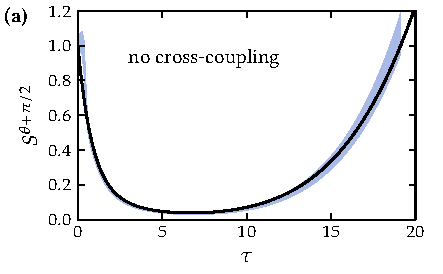
\includegraphics{figures_generated/exact/squeezing_nocc_100.pdf}%
    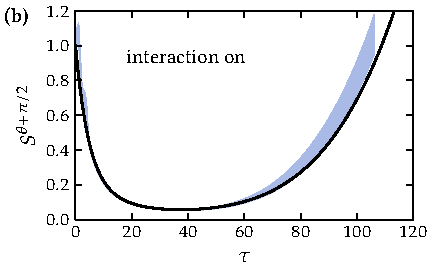
\includegraphics{figures_generated/exact/squeezing_cc_100.pdf}}

    \caption{
    Comparison of the Wigner simulated time-dependent local squeezing (blue bands; the width corresponds to the estimated sampling error) against the exact results (black lines).
    Trajectories used: $2000$.
    The plots correspond to \textbf{(a)} $\tilde{g}_{12} = 0$, and \textbf{(b)} $\tilde{g}_{12} \approx 1 / N_A$.}

    \label{fig:wigner-bec:mm:squeezing-comparison}
\end{figure}

\begin{figure}
    \centerline{%
    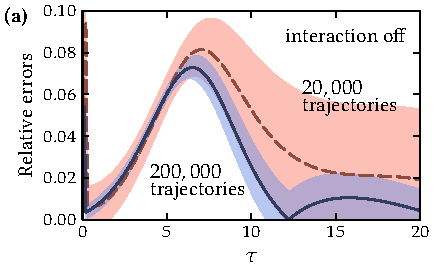
\includegraphics{figures_generated/exact/squeezing_nocc_err.pdf}%
    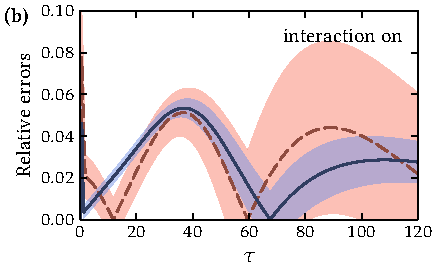
\includegraphics{figures_generated/exact/squeezing_cc_err.pdf}}

    \caption{
    Difference of the Wigner simulated local squeezing and the exact results (solid lines) as compared to the sampling errors in Wigner simulations (dashed lines).
    Plotted are the results for $2000$ trajectories (blue lines) and $20000$ trajectories (red lines).
    The plots correspond to \textbf{(a)} $\tilde{g}_{12} = 0$, and \textbf{(b)} $\tilde{g}_{12} \approx 1 / N_A$.}

    \label{fig:wigner-bec:mm:squeezing-error-comparison}
\end{figure}

The expectations above can be expressed in terms of creation and annihilation operators, and calculated either in Wigner representation using \thmref{mm-wigner:mm:moments}, or with the number state expansion using~\eqnref{wigner-bec:mm:exact-a} and~\eqnref{wigner-bec:mm:exact-f} (courtesy of Q.~Y.~He).
The results are plotted in~\figref{wigner-bec:mm:squeezing-comparison}.
The Wigner method shows good agreement with the exact results in the time range of interest; the growing sampling error can be reduced to a desirable extent by using more simulation trajectories.
Nevertheless, the Wigner results show a systematic error (\figref{wigner-bec:mm:squeezing-error-comparison}), which is inside the sampling error range for the low number of trajectories, but preserves its magnitude as the number of trajectories is increased (and the sampling error decreased).
This is a sign of the failing truncation approximation.
The large oscillations of the systematic error at the start of the simulation can be explained by accumulating uncertainties in the denominator of~\eqnref{wigner-bec:mm:squeezing}.

Note that while in this particular example the exact method gives more accurate results at comparable or lower computational cost, it becomes unapplicable as soon as one wants to include tunneling and nonlinear losses into the model, while the Wigner method continues to perform with the same effectiveness~\cite{Opanchuk2012a}.

